\documentclass[a4paper,11pt]{report}
\usepackage[T1]{fontenc}
\usepackage[utf8]{inputenc}
\usepackage{lmodern}
\usepackage{booktabs}
\usepackage[margin=3.5cm]{geometry}
\usepackage{color, colortbl}
\usepackage{graphicx}
\usepackage[binary-units=true]{siunitx}  

\definecolor{Gray}{gray}{0.9}

\title{MiloSAR Documentation \\ \vspace{0.5cm} \Large Version 0.1}
\author{Darryn Jordan}

\begin{document}

\maketitle
\tableofcontents

\chapter{Introduction}

\chapter{Synthesizer}

\section{$ \mu $Wire Interface}

The LMX2492EVM is packaged with a USBtoMANY converter, enabling users to program the evaluation module through its $ \mu $Wire connector using TI's CodeLoader. This process is however tedious, especially when programming two synthesizers with different waveforms. The LMX2492 datasheet provides the timing requirements and clocking structure for programming the synthesizer through its $ \mu $Wire connector pins. GPIO pins on the Red Pitaya were used to program both synthesizers efficiently. Figure~\ref{fig_rp_synth_connect} illustrates the connection between the Red Pitaya and two LMX2492 evaluation boards.
\begin{figure}[h!]
    \begin{center}
        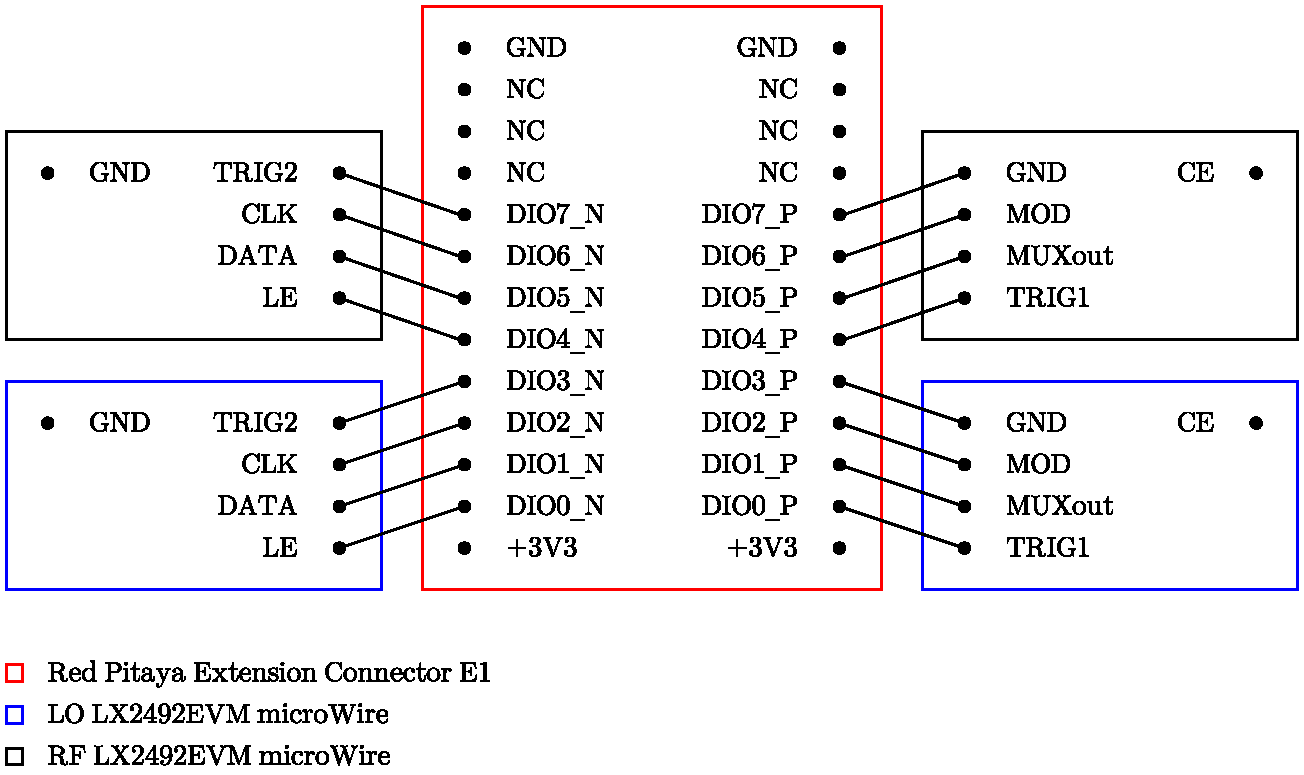
\includegraphics[width=\textwidth]{images/rp_synth_connections.pdf}
        \caption{Wiring diagram for connection between Red Pitaya and the LMX2492.}
        \label{fig_rp_synth_connect}
    \end{center}
\end{figure}

\chapter{FPGA}

\section{Registers}

\subsection{Configuration}
The configuration register is currently only used to set the decimation factor for reducing sampling rate. Sixteen bits are reserved for later use.
\begin{table}[ht]
    \caption{General configuration register.}
    \begin{center}
        \begin{tabular}{|c|c|c|c|c|c|c|c|c|c|c|c|c|c|c|c|}
            \hline
            \rowcolor{Gray}
            \multicolumn{8}{|c|}{B3} & \multicolumn{8}{c|}{B2}\\
            \hline
            31 & 30 & 29 & 28 & 27 & 26 & 25 & 24 & 23 & 22 & 21 & 20 & 19 & 18 & 17 & 16 \\
            \hline
            \multicolumn{8}{|c|}{Reserved [31:24]} & \multicolumn{8}{c|}{Reserved [23:16]}\\
            \hline  
            
            \addlinespace[0.5cm]
            
            \hline 
            \rowcolor{Gray}
            \multicolumn{8}{|c|}{B1} & \multicolumn{8}{c|}{B0}\\
            \hline
            15 & 14 & 13 & 12 & 11 & 10 & 9 & 8 & 7 & 6 & 5 & 4 & 3 & 2 & 1 & 0 \\
            \hline
            \multicolumn{16}{|c|}{Decimation Factor [15:0]}\\
            \hline
        \end{tabular}
    \end{center}
    \label{tab:config_reg}
\end{table}

\subsection{Channel X Status}
Both recording channels within the FPGA require a status register to provide the CPU with the location of the RAM writer's current pointer location.
\begin{table}[ht]
    \caption{Channel X status register.}
    \begin{center}
        \begin{tabular}{|c|c|c|c|c|c|c|c|c|c|c|c|c|c|c|c|}
            \hline
            \rowcolor{Gray}
            \multicolumn{8}{|c|}{B3} & \multicolumn{8}{c|}{B2}\\
            \hline
            31 & 30 & 29 & 28 & 27 & 26 & 25 & 24 & 23 & 22 & 21 & 20 & 19 & 18 & 17 & 16 \\
            \hline
            \multicolumn{16}{|c|}{Channel X Pointer [31:16]}\\
            \hline  
            
            \addlinespace[0.5cm]
            
            \hline 
            \rowcolor{Gray}
            \multicolumn{8}{|c|}{B1} & \multicolumn{8}{c|}{B0}\\
            \hline
            15 & 14 & 13 & 12 & 11 & 10 & 9 & 8 & 7 & 6 & 5 & 4 & 3 & 2 & 1 & 0 \\
            \hline
            \multicolumn{16}{|c|}{Channel X Pointer [15:0]}\\
            \hline
        \end{tabular}
    \end{center}
    \label{tab:status_reg}
\end{table}

\subsection{Synthesizer Reference Signal}
Provides the FPGA with the DDS phase increment used to generate the \SI{50}{\MHz} phase reference signal.
\begin{table}[ht]
    \caption{Synthesizer reference signal phase increment register.}
    \begin{center}
        \begin{tabular}{|c|c|c|c|c|c|c|c|c|c|c|c|c|c|c|c|}
            \hline
            \rowcolor{Gray}
            \multicolumn{8}{|c|}{B3} & \multicolumn{8}{c|}{B2}\\
            \hline
            31 & 30 & 29 & 28 & 27 & 26 & 25 & 24 & 23 & 22 & 21 & 20 & 19 & 18 & 17 & 16 \\
            \hline
            \multicolumn{16}{|c|}{Phase Increment [31:16]}\\
            \hline  
            
            \addlinespace[0.5cm]
            
            \hline 
            \rowcolor{Gray}
            \multicolumn{8}{|c|}{B1} & \multicolumn{8}{c|}{B0}\\
            \hline
            15 & 14 & 13 & 12 & 11 & 10 & 9 & 8 & 7 & 6 & 5 & 4 & 3 & 2 & 1 & 0 \\
            \hline
            \multicolumn{16}{|c|}{Phase Increment [15:0]}\\
            \hline
        \end{tabular}
    \end{center}
    \label{tab:ref_phase_inc}
\end{table}

\subsection{GPIO}

\begin{table}[ht]
    \caption{GPIO register.}
    \begin{center}
        \begin{tabular}{|c|c|c|c|c|c|c|c|c|c|c|c|c|c|c|c|}
            \hline
            \rowcolor{Gray}
            \multicolumn{8}{|c|}{B3} & \multicolumn{8}{c|}{B2}\\
            \hline
            31 & 30 & 29 & 28 & 27 & 26 & 25 & 24 & 23 & 22 & 21 & 20 & 19 & 18 & 17 & 16 \\
            \hline
            \multicolumn{16}{|c|}{Clock Divisor [31:16]}\\
            \hline  
            
            \addlinespace[0.5cm]
            
            \hline 
            \rowcolor{Gray}
            \multicolumn{8}{|c|}{B1} & \multicolumn{8}{c|}{B0}\\
            \hline
            15 & 14 & 13 & 12 & 11 & 10 & 9 & 8 & 7 & 6 & 5 & 4 & 3 & 2 & 1 & 0 \\
            \hline
            \multicolumn{7}{|c|}{Clock Divisor [15:9]} & E & \multicolumn{8}{c|}{GPION [7:0]}\\
            \hline
        \end{tabular}
    \end{center}
    \label{tab:gpio_reg}
\end{table}

\subsection{Cancellation}

\begin{table}[ht]
    \caption{Cancellation signal phase increment register.}
    \begin{center}
        \begin{tabular}{|c|c|c|c|c|c|c|c|c|c|c|c|c|c|c|c|}
            \hline
            \rowcolor{Gray}
            \multicolumn{8}{|c|}{B3} & \multicolumn{8}{c|}{B2}\\
            \hline
            31 & 30 & 29 & 28 & 27 & 26 & 25 & 24 & 23 & 22 & 21 & 20 & 19 & 18 & 17 & 16 \\
            \hline
            \multicolumn{16}{|c|}{Phase Increment [31:16]}\\
            \hline  
            
            \addlinespace[0.5cm]
            
            \hline 
            \rowcolor{Gray}
            \multicolumn{8}{|c|}{B1} & \multicolumn{8}{c|}{B0}\\
            \hline
            15 & 14 & 13 & 12 & 11 & 10 & 9 & 8 & 7 & 6 & 5 & 4 & 3 & 2 & 1 & 0 \\
            \hline
            \multicolumn{16}{|c|}{Phase Increment [15:0]}\\
            \hline
        \end{tabular}
    \end{center}
    \label{tab:canc_phase_inc}
\end{table}


\end{document}
